\documentclass[11pt,a4paper]{article}
\usepackage[margin=2.5cm]{geometry}
\usepackage{graphicx}
\usepackage{xcolor}
\usepackage{tikz}
\usepackage{amsmath}
\usepackage{amssymb}
\usepackage{enumitem}
\usepackage{tcolorbox}
\usepackage{multicol}
\usepackage{fancyhdr}
\usepackage{hyperref}

% Define colors from slides
\definecolor{mlblue}{HTML}{1f77b4}
\definecolor{mlorange}{HTML}{ff7f0e}
\definecolor{mlgreen}{HTML}{2ca02c}
\definecolor{mlred}{HTML}{d62728}
\definecolor{mlpurple}{HTML}{9467bd}
\definecolor{mlgray}{HTML}{7f7f7f}

% TikZ libraries
\usetikzlibrary{shapes.geometric, arrows, positioning, calc}

% Page style
\pagestyle{fancy}
\fancyhf{}
\lhead{\textcolor{mlblue}{\textbf{ML for Innovation}}}
\rhead{\textcolor{mlgray}{Week 1: Discovery Handout}}
\cfoot{\thepage}
\renewcommand{\headrulewidth}{0.4pt}

% Custom environments
\newtcolorbox{discoverybox}[2]{
    colback=#1!10, 
    colframe=#1!50, 
    title={#2}
}

\newtcolorbox{exercisebox}[2]{
    colback=white, 
    colframe=#1!50, 
    title={Exercise: #2}
}

\newcommand{\thinkbox}[1]{
\begin{tcolorbox}[colback=yellow!10, colframe=mlorange!70, title={Think About This}]
#1
\end{tcolorbox}
}

\begin{document}

% PAGE 1: Cover Page
\thispagestyle{empty}
\begin{center}
\vspace*{2cm}

{\Huge \textcolor{mlblue}{\textbf{Machine Learning for Innovation}}}

\vspace{1cm}

{\LARGE \textcolor{mlpurple}{A Discovery Journey}}

\vspace{2cm}

{\Large Week 1: Finding Patterns in Chaos}

\vspace{1cm}

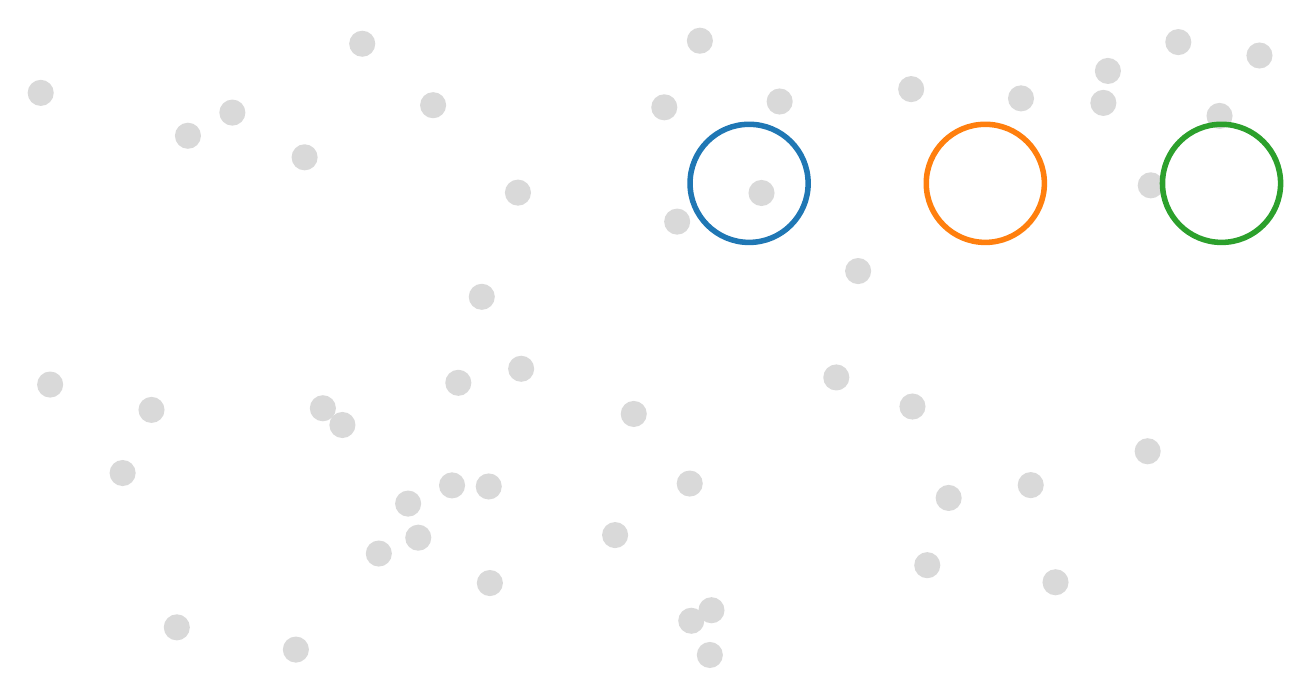
\begin{tikzpicture}
% Draw scattered points to represent chaos
\foreach \i in {1,...,50} {
    \pgfmathsetmacro{\xpos}{rand*8}
    \pgfmathsetmacro{\ypos}{rand*4}
    \node[circle, fill=gray!30, minimum size=3pt] at (\xpos,\ypos) {};
}
% Draw three clusters
\node[circle, draw=mlblue, line width=2pt, minimum size=1.5cm] at (1,2) {};
\node[circle, draw=mlorange, line width=2pt, minimum size=1.5cm] at (4,2) {};
\node[circle, draw=mlgreen, line width=2pt, minimum size=1.5cm] at (7,2) {};
\end{tikzpicture}

\vspace{3cm}

\begin{tcolorbox}[colback=white, colframe=mlblue!50, width=0.7\textwidth]
\Large
\textbf{Name:} \hrulefill

\vspace{0.5cm}

\textbf{Date:} \hrulefill
\end{tcolorbox}

\end{center}

\newpage

% PAGE 2: Innovation Challenge Discovery
\section*{Page 2: The Innovation Challenge}

\begin{discoverybox}{mlblue}{Your Innovation Universe}
Think about innovations in your field. They could be products, services, processes, or ideas.
\end{discoverybox}

\begin{exercisebox}{mlorange}{Draw Your Innovation Ideas}
In the grid below, place 20 different innovation ideas as dots. Don't think too hard - just scatter them naturally.

\begin{center}
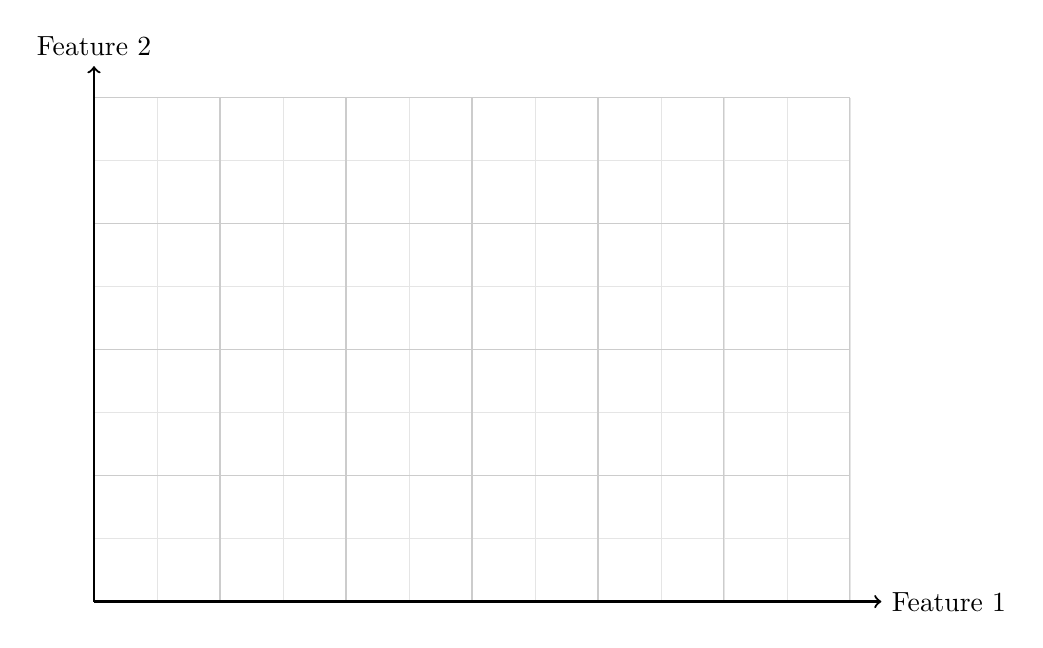
\begin{tikzpicture}[scale=0.8]
% Draw grid
\draw[step=1cm, gray!20, very thin] (0,0) grid (12,8);
\draw[step=2cm, gray!40, thin] (0,0) grid (12,8);
% Add axes
\draw[->, thick] (0,0) -- (12.5,0) node[right] {Feature 1};
\draw[->, thick] (0,0) -- (0,8.5) node[above] {Feature 2};
\end{tikzpicture}
\end{center}
\end{exercisebox}

\vspace{1cm}

\begin{discoverybox}{mlgreen}{Discovery Questions}
\begin{enumerate}[itemsep=0.5cm]
\item Look at your dots. Can you see any natural groups? Circle them.
\vspace{1cm}
\item What makes grouping difficult? List three challenges:
\begin{itemize}
\item \hrulefill
\item \hrulefill
\item \hrulefill
\end{itemize}
\vspace{0.5cm}
\item Why might a computer be better at finding these patterns?
\vspace{1cm}
\hrulefill

\hrulefill
\end{enumerate}
\end{discoverybox}

\thinkbox{
\textbf{Key Insight:} Human brains can only visualize 2-3 dimensions at once. But innovations have hundreds of features!
}

\newpage

% PAGE 3: Feature Complexity Exploration
\section*{Page 3: The Hidden Dimensions}

\begin{exercisebox}{mlpurple}{Feature Discovery}
Pick ONE innovation idea (e.g., a smart home device, an app, a new service). Write it here:

\textbf{My Innovation:} \hrulefill

Now, list ALL the factors that could affect its success:
\end{exercisebox}

\begin{multicols}{2}
\begin{discoverybox}{mlblue}{Technical Features}
\begin{itemize}[itemsep=0.3cm]
\item \hrulefill
\item \hrulefill
\item \hrulefill
\item \hrulefill
\item \hrulefill
\end{itemize}
\end{discoverybox}

\begin{discoverybox}{mlorange}{Market Features}
\begin{itemize}[itemsep=0.3cm]
\item \hrulefill
\item \hrulefill
\item \hrulefill
\item \hrulefill
\item \hrulefill
\end{itemize}
\end{discoverybox}

\begin{discoverybox}{mlgreen}{User Features}
\begin{itemize}[itemsep=0.3cm]
\item \hrulefill
\item \hrulefill
\item \hrulefill
\item \hrulefill
\item \hrulefill
\end{itemize}
\end{discoverybox}

\begin{discoverybox}{mlred}{Financial Features}
\begin{itemize}[itemsep=0.3cm]
\item \hrulefill
\item \hrulefill
\item \hrulefill
\item \hrulefill
\item \hrulefill
\end{itemize}
\end{discoverybox}
\end{multicols}

\begin{exercisebox}{mlpurple}{Dimension Realization}
\begin{enumerate}
\item How many total features did you identify? \hrulefill
\item If each innovation has this many features, how would you compare 1000 innovations?
\vspace{1cm}
\hrulefill
\item This is why we need Machine Learning! It can handle hundreds of dimensions that we can't visualize.
\end{enumerate}
\end{exercisebox}

\newpage

% PAGE 4: K-Means Discovery Activity
\section*{Page 4: Discovering K-Means Clustering}

\begin{exercisebox}{mlblue}{Manual Clustering Challenge}
You'll now experience what the K-Means algorithm does!

\textbf{Step 1:} Place 3 center points (marked with X) anywhere on the grid with dots:
\end{exercisebox}

\begin{center}
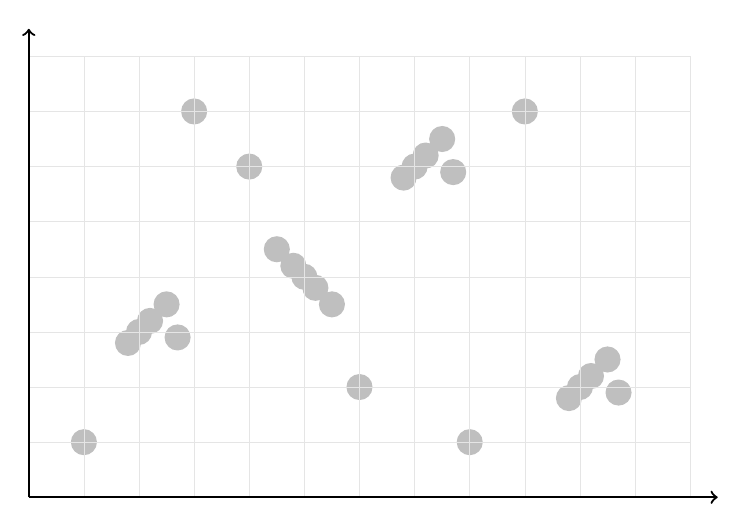
\begin{tikzpicture}[scale=0.7]
% Pre-place some data points
\foreach \point in {
    (2,3), (2.5,3.5), (1.8,2.8), (2.2,3.2), (2.7,2.9),
    (7,6), (7.5,6.5), (6.8,5.8), (7.2,6.2), (7.7,5.9),
    (10,2), (10.5,2.5), (9.8,1.8), (10.2,2.2), (10.7,1.9),
    (5,4), (4.5,4.5), (5.5,3.5), (4.8,4.2), (5.2,3.8),
    (3,7), (8,1), (1,1), (9,7), (6,2), (4,6)
} {
    \node[circle, fill=gray!50, minimum size=4pt] at \point {};
}
% Grid
\draw[step=1cm, gray!20, very thin] (0,0) grid (12,8);
\draw[->, thick] (0,0) -- (12.5,0);
\draw[->, thick] (0,0) -- (0,8.5);
\end{tikzpicture}
\end{center}

\begin{exercisebox}{mlorange}{K-Means Steps}
\textbf{Step 2:} For each dot, draw a line to its nearest center (X).

\textbf{Step 3:} Count how many dots belong to each center:
\begin{itemize}
\item Center 1: \_\_\_\_ dots
\item Center 2: \_\_\_\_ dots  
\item Center 3: \_\_\_\_ dots
\end{itemize}

\textbf{Step 4:} Now move each X to the middle of its assigned dots (this is the ``mean'' in K-means!).

\textbf{Step 5:} Would you need to repeat? Why?
\vspace{1cm}
\hrulefill
\end{exercisebox}

\begin{discoverybox}{mlgreen}{What Happens When K Changes?}
\begin{enumerate}
\item What if you used K=2 centers instead? Draw how the groups would change.
\item What if K=5? Would that be better or worse? Why?
\vspace{1cm}
\hrulefill
\end{enumerate}
\end{discoverybox}

\newpage

% PAGE 5: Distance Metrics Exploration
\section*{Page 5: How Do We Measure ``Close''?}

\begin{exercisebox}{mlblue}{Distance Discovery}
Consider two innovation ideas with features:
\begin{itemize}
\item Innovation A: (x=2, y=3)
\item Innovation B: (x=5, y=7)
\end{itemize}
\end{exercisebox}

\begin{multicols}{2}
\begin{discoverybox}{mlorange}{Euclidean Distance}
``As the crow flies'' - straight line

\textbf{Formula:} $d = \sqrt{(x_2-x_1)^2 + (y_2-y_1)^2}$

\textbf{Calculate:}
\begin{align*}
d &= \sqrt{(5-2)^2 + (7-3)^2}\\
&= \sqrt{\_\_\_\_ + \_\_\_\_}\\
&= \sqrt{\_\_\_\_}\\
&= \_\_\_\_
\end{align*}

\textbf{When to use:} Physical measurements
\end{discoverybox}

\begin{discoverybox}{mlgreen}{Manhattan Distance}
``City blocks'' - grid walking

\textbf{Formula:} $d = |x_2-x_1| + |y_2-y_1|$

\textbf{Calculate:}
\begin{align*}
d &= |5-2| + |7-3|\\
&= \_\_\_\_ + \_\_\_\_\\
&= \_\_\_\_
\end{align*}

\textbf{When to use:} Features are independent
\end{discoverybox}
\end{multicols}

\begin{exercisebox}{mlpurple}{Distance in Innovation Context}
\begin{enumerate}
\item If x = ``development cost'' and y = ``time to market'', which distance makes more sense?

\hrulefill

\item If you had 100 features instead of 2, could you still calculate distance?

\hrulefill

\item Draw the two different distance paths on this grid:
\end{enumerate}
\end{exercisebox}

\begin{center}
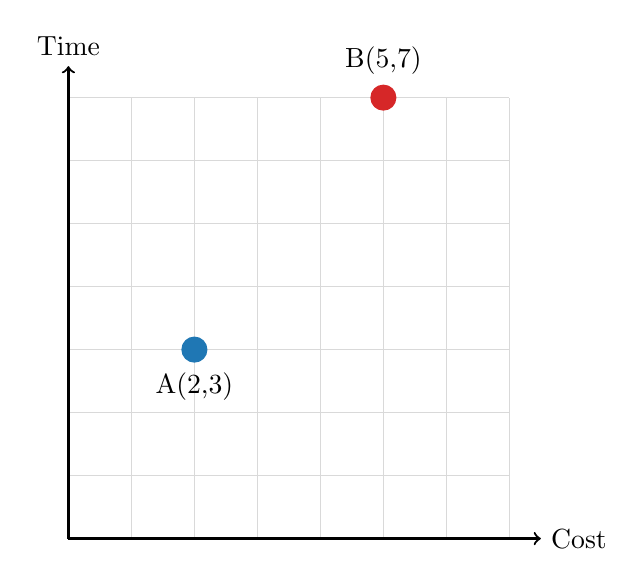
\begin{tikzpicture}[scale=0.8]
\draw[step=1cm, gray!30, thin] (0,0) grid (7,7);
\node[circle, fill=mlblue, minimum size=6pt, label=below:{A(2,3)}] at (2,3) {};
\node[circle, fill=mlred, minimum size=6pt, label=above:{B(5,7)}] at (5,7) {};
\draw[->, thick] (0,0) -- (7.5,0) node[right] {Cost};
\draw[->, thick] (0,0) -- (0,7.5) node[above] {Time};
\end{tikzpicture}
\end{center}

\newpage

% PAGE 6: Quality Measurement Discovery
\section*{Page 6: How Good Are Your Clusters?}

\begin{discoverybox}{mlblue}{The Silhouette Score}
Measures how well-separated your clusters are (ranges from -1 to 1).
\end{discoverybox}

\begin{exercisebox}{mlorange}{Calculate Your Own Silhouette}
Look at this simple example with 3 clusters:

\begin{center}
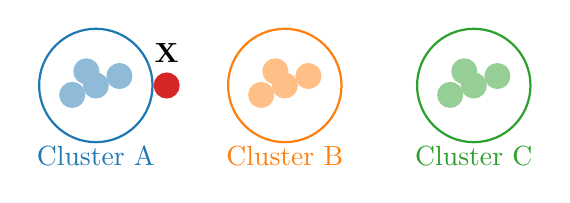
\begin{tikzpicture}[scale=0.6]
% Cluster 1
\draw[mlblue, thick] (1,1) circle (1.2cm);
\foreach \point in {(0.5,0.8), (1,1), (1.5,1.2), (0.8,1.3)} {
    \node[circle, fill=mlblue!50, minimum size=4pt] at \point {};
}
\node[mlblue] at (1,-0.5) {Cluster A};

% Cluster 2
\draw[mlorange, thick] (5,1) circle (1.2cm);
\foreach \point in {(4.5,0.8), (5,1), (5.5,1.2), (4.8,1.3)} {
    \node[circle, fill=mlorange!50, minimum size=4pt] at \point {};
}
\node[mlorange] at (5,-0.5) {Cluster B};

% Cluster 3
\draw[mlgreen, thick] (9,1) circle (1.2cm);
\foreach \point in {(8.5,0.8), (9,1), (9.5,1.2), (8.8,1.3)} {
    \node[circle, fill=mlgreen!50, minimum size=4pt] at \point {};
}
\node[mlgreen] at (9,-0.5) {Cluster C};

% One test point
\node[circle, fill=mlred, minimum size=8pt, label=above:{\textbf{X}}] at (2.5,1) {};
\end{tikzpicture}
\end{center}

For point X:
\begin{itemize}
\item a(X) = average distance to points in same cluster = \_\_\_\_
\item b(X) = average distance to points in nearest other cluster = \_\_\_\_
\item Silhouette(X) = $\frac{b(X) - a(X)}{\max(a(X), b(X))}$ = \_\_\_\_
\end{itemize}
\end{exercisebox}

\begin{exercisebox}{mlgreen}{Interpret the Score}
\begin{itemize}
\item Score close to 1: \hrulefill (Well/Poorly) clustered
\item Score close to 0: \hrulefill (On the border/In the center)
\item Score close to -1: \hrulefill (Correct/Wrong) cluster
\end{itemize}
\end{exercisebox}

\begin{discoverybox}{mlpurple}{The Elbow Method}
Plot the ``cost'' (sum of distances) vs. number of clusters:

\begin{center}
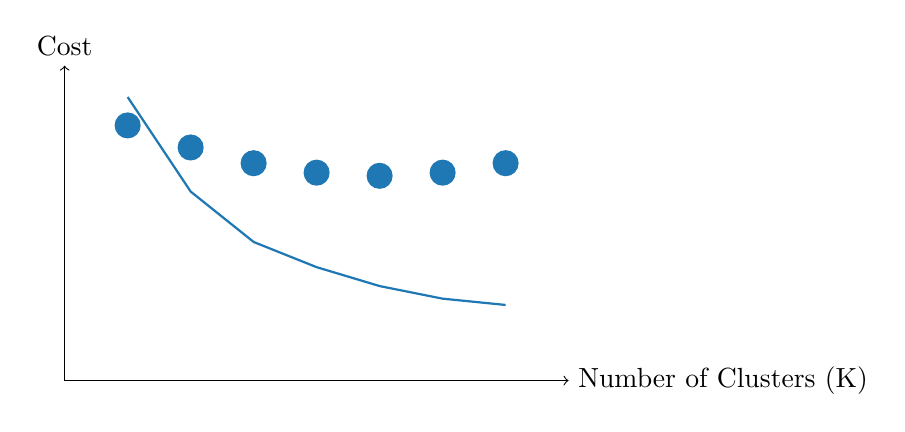
\begin{tikzpicture}[scale=0.8]
\draw[->] (0,0) -- (8,0) node[right] {Number of Clusters (K)};
\draw[->] (0,0) -- (0,5) node[above] {Cost};
% Draw elbow curve
\draw[thick, mlblue] (1,4.5) -- (2,3) -- (3,2.2) -- (4,1.8) -- (5,1.5) -- (6,1.3) -- (7,1.2);
\foreach \x in {1,...,7} {
    \node[circle, fill=mlblue, minimum size=4pt] at (\x, {4.5 - 0.5*\x + 0.05*\x*\x}) {};
}
\end{tikzpicture}
\end{center}

Circle where you think the ``elbow'' is. This is your optimal K!
\end{discoverybox}

\newpage

% PAGE 7: Algorithm Selection Guide
\section*{Page 7: Choosing the Right Algorithm}

\begin{exercisebox}{mlblue}{Build Your Decision Tree}
Fill in the blanks to create your algorithm selection guide:
\end{exercisebox}

\begin{center}
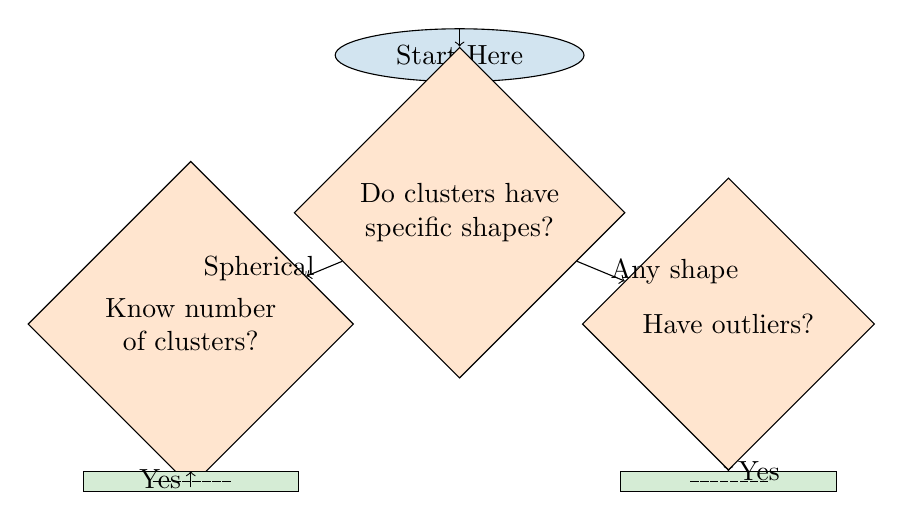
\begin{tikzpicture}[
    node distance=2cm,
    decision/.style={diamond, draw, text width=3cm, align=center, fill=mlorange!20},
    algo/.style={rectangle, draw, text width=2.5cm, align=center, fill=mlgreen!20},
    start/.style={ellipse, draw, text width=2cm, align=center, fill=mlblue!20}
]

\node[start] (start) {Start Here};
\node[decision, below of=start] (shape) {Do clusters have specific shapes?};
\node[decision, below left of=shape, xshift=-2cm] (know) {Know number of clusters?};
\node[decision, below right of=shape, xshift=2cm] (noise) {Have outliers?};
\node[algo, below of=know] (kmeans) {\_\_\_\_\_\_\_\_};
\node[algo, below of=noise] (dbscan) {\_\_\_\_\_\_\_\_};

\draw[->] (start) -- (shape);
\draw[->] (shape) -- node[left] {Spherical} (know);
\draw[->] (shape) -- node[right] {Any shape} (noise);
\draw[->] (know) -- node[left] {Yes} (kmeans);
\draw[->] (noise) -- node[right] {Yes} (dbscan);

\end{tikzpicture}
\end{center}

\begin{exercisebox}{mlorange}{Match the Scenario}
Draw lines connecting scenarios to the best algorithm:

\begin{multicols}{2}
\textbf{Scenarios:}
\begin{enumerate}
\item Customer segments (equal size)
\item Finding fraud (rare events)
\item Product categories (hierarchy)
\item Geographic regions (density)
\item User behaviors (overlapping)
\end{enumerate}

\columnbreak

\textbf{Algorithms:}
\begin{itemize}
\item K-Means
\item DBSCAN
\item Hierarchical
\item Gaussian Mixture
\item Mean Shift
\end{itemize}
\end{multicols}
\end{exercisebox}

\begin{discoverybox}{mlred}{Your Innovation Context}
Which algorithm would work best for YOUR innovation challenge? Why?

\vspace{2cm}
\hrulefill

\hrulefill
\end{discoverybox}

\newpage

% PAGE 8: Innovation Application Planning
\section*{Page 8: Your Innovation Clustering Project}

\begin{exercisebox}{mlpurple}{Design Your Project}
Now apply everything you've learned to a real innovation challenge!
\end{exercisebox}

\begin{discoverybox}{mlblue}{1. Define Your Innovation Dataset}
\textbf{What innovations will you analyze?} (products, services, ideas, etc.)

\hrulefill

\textbf{How many items?} \_\_\_\_\_\_

\textbf{List 5 key features you'll measure:}
\begin{enumerate}
\item \hrulefill
\item \hrulefill
\item \hrulefill
\item \hrulefill
\item \hrulefill
\end{enumerate}
\end{discoverybox}

\begin{discoverybox}{mlorange}{2. Choose Your Method}
\textbf{Which clustering algorithm?} \hrulefill

\textbf{Why this one?} 

\hrulefill

\hrulefill

\textbf{How many clusters (K) do you expect?} \_\_\_\_\_\_ 

\textbf{Why?} \hrulefill
\end{discoverybox}

\begin{discoverybox}{mlgreen}{3. Define Success}
\textbf{What silhouette score would be ``good enough''?} \_\_\_\_\_\_

\textbf{How will you validate your clusters make business sense?}

\hrulefill

\hrulefill
\end{discoverybox}

\begin{discoverybox}{mlred}{4. Reflection}
\textbf{Three things I discovered about clustering today:}
\begin{enumerate}
\item \hrulefill
\item \hrulefill
\item \hrulefill
\end{enumerate}

\textbf{One question I still have:}

\hrulefill

\textbf{How I'll use this in my innovation work:}

\hrulefill

\hrulefill
\end{discoverybox}

\vspace{1cm}

\begin{center}
\begin{tcolorbox}[colback=mlpurple!10, colframe=mlpurple!50, width=0.8\textwidth]
\centering
\Large \textbf{Congratulations!}\\[0.5cm]
\normalsize You've discovered the fundamentals of clustering for innovation.\\
Next week: Advanced clustering techniques!
\end{tcolorbox}
\end{center}

\end{document}